\chapter{Experiments}

\section{Preload}
The preload experiment is defined by a force or stress value and by the velocity. The velocity can be chosen as either in \(mm/sec\) or by \(\% length_{mounting}/sec\), as shown in figure \ref{fig:preload}. If one velocity input changes, the other will adapt accordingly.
\\
\\
In a preload experiment, the sample will be stretched with the defined velocity until the defined force/stress is reached and then the stage stops at this position.

\begin{figure}[!ht]
	\centering
		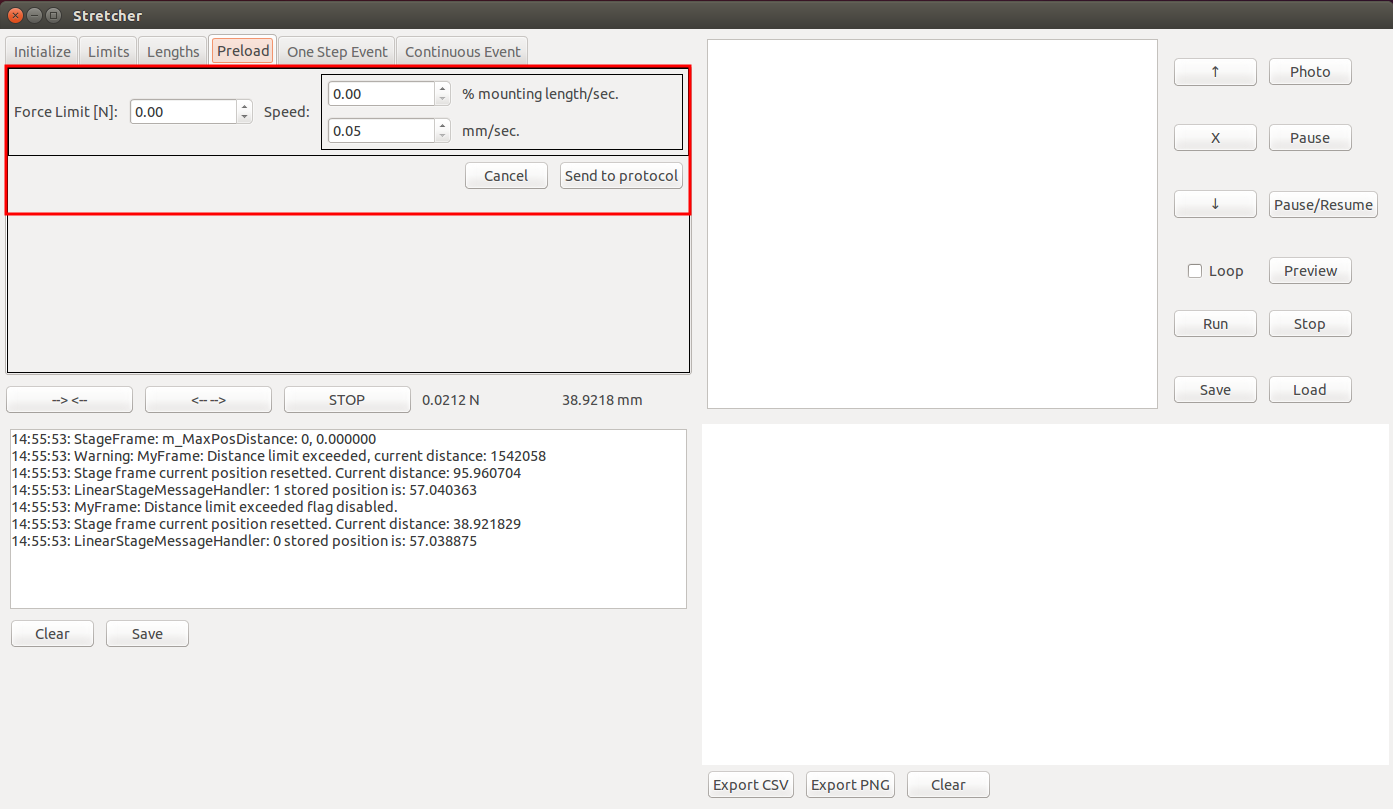
\includegraphics[width=1.0\textwidth]{images/Preload}
	\caption{Preload experiment}
	\label{fig:preload}
\end{figure}

\section{One step event}
The one step event is either distance based, as shown in figure \ref{fig:onestepeventdistance}, or force/stress based, as shown in figure \ref{fig:onestepeventforcestress}. In both cases, the experiment is defined by a velocity (mm/s or \(\%L_{0}/sec\)), a delay time, a limit and a dwell time. The experiment can be repeated by checking the check-box "Repeat" and inserting a cycle number. The behavior at the end of the experiment can also be selected. The following options are possible: Stop, Hold a distance, Go to \(L_{0}\) and Go to \(length_{mounting}\). The distance limit and the hold distance can both be defined in three ways, either by mm relative to the start length, mm absolute or by \(\%L_{0}\).
\\
\\
In the one step event experiment, the sample will be stretched with the defined velocity until the limit is reached, after the delay time is over. After the limit is reached, the experiment waits until the dwell time is over and after repeat these steps or act as defined in the end of event behavior, if it was the last cycle.

\begin{figure}[!ht]
	\centering
		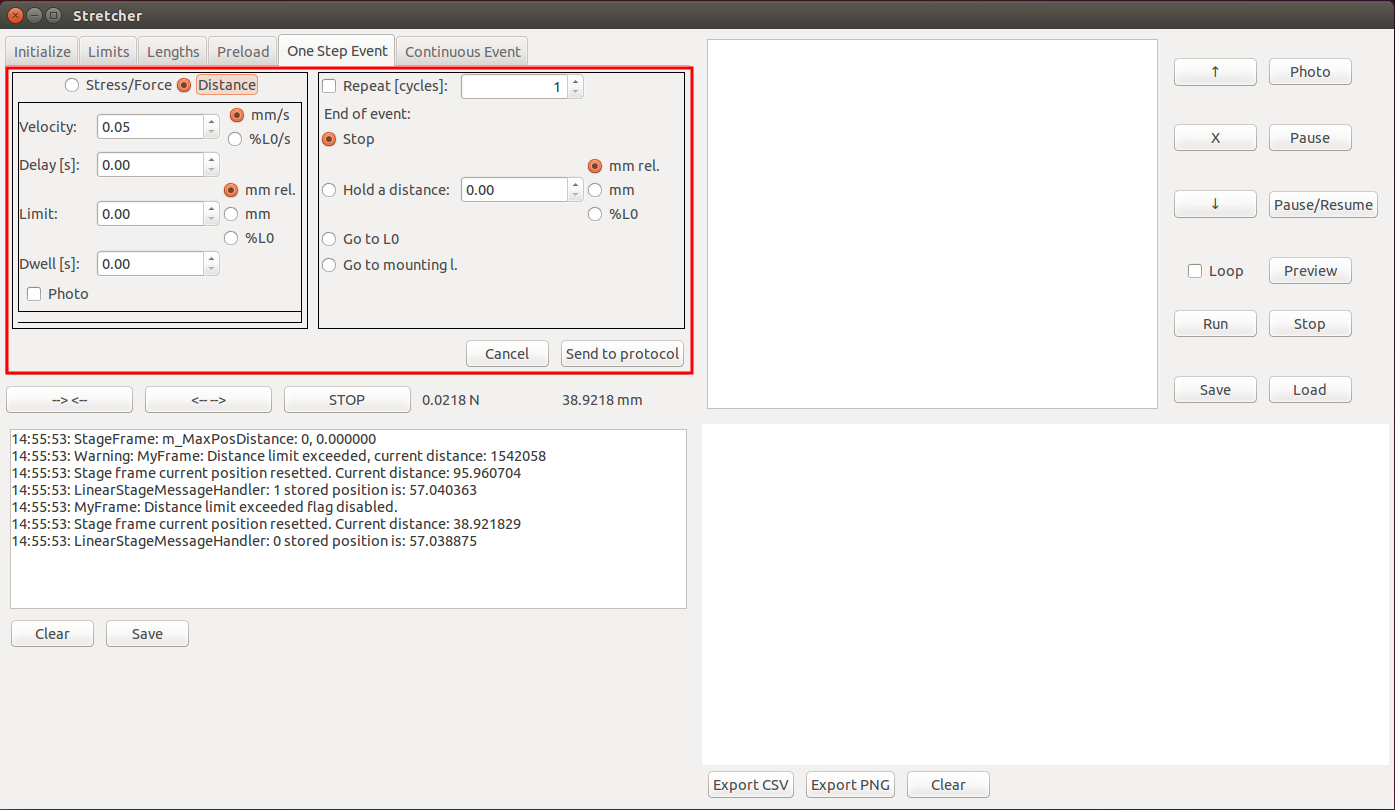
\includegraphics[width=1.0\textwidth]{images/OneStepEventDistance}
	\caption{One step event experiment distance based}
	\label{fig:onestepeventdistance}
\end{figure}

\begin{figure}[!ht]
	\centering
		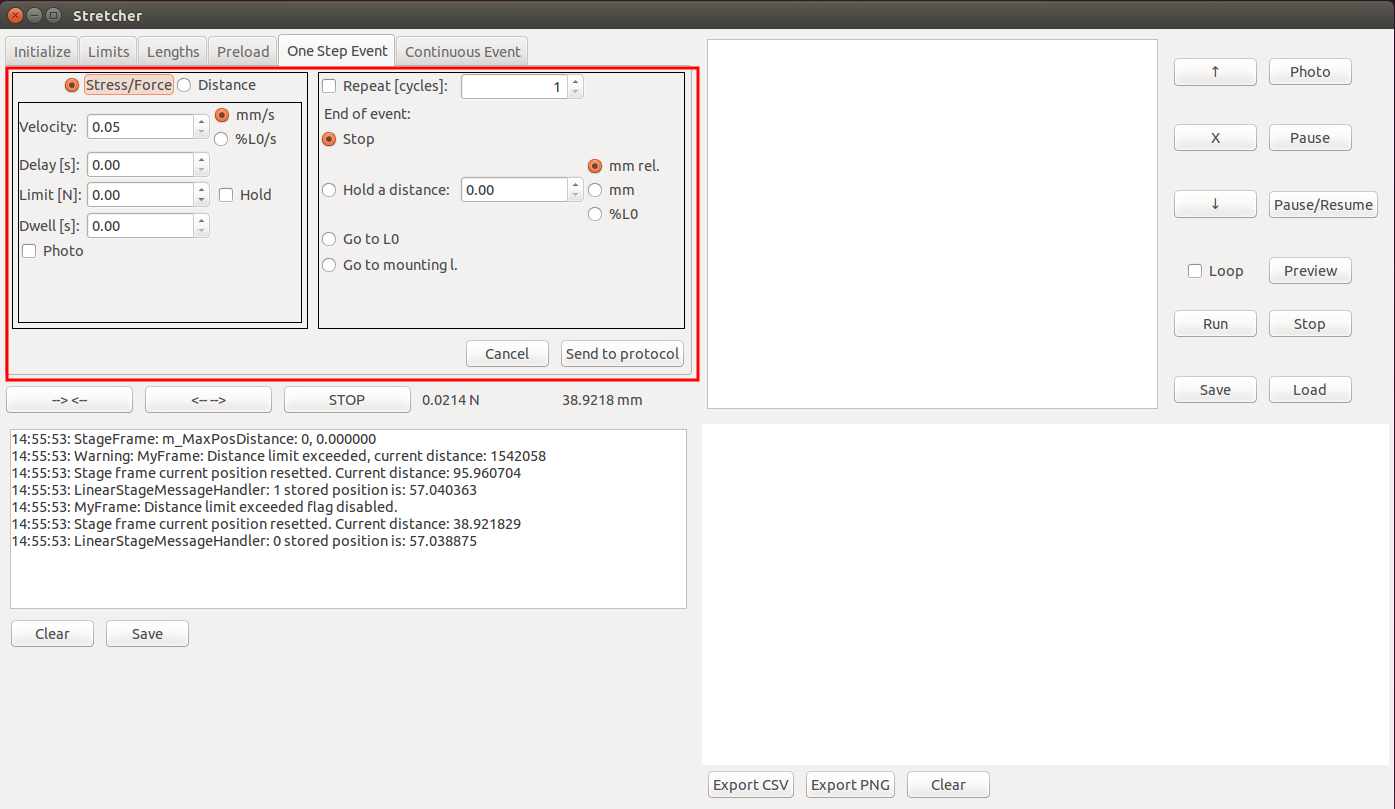
\includegraphics[width=1.0\textwidth]{images/OneStepEventStressForce}
	\caption{One step event experiment force/stress based}
	\label{fig:onestepeventforcestress}
\end{figure}

\section{Continuous event}
The continuous event is also either distance based, as shown in figure \ref{fig:continuouseventdistance}, or force/stress based, as shown in figure \ref{fig:continuouseventforcestress}. In both cases, the experiment is defined by a velocity (mm/s or \(\%L_{0}\)), a hold time, an increment and a maximal value or a number of steps. The experiment can also be repeated by checking the check-box "Repeat" and inserting a cycle number. The behavior at the end of the experiment can also be selected. The following options are possible: Stop, Go to \(L_{0}\), Go to \(length_{mounting}\) and Stop at force/stress. The distance increment can be defined in two ways, either by mm absolute or by \(\%L_{0}\). The distance maximal value can be defined in three ways as the increment or by mm relative to the start length. If the experiment is defined by a maximal value, the steps will be calculated at the start of the experiment otherwise the inserted steps will be taken into account. If the maximal value is defined in \(\%F_{max}\) a ramp to failure experiment will be performed and the increment values will be ignored.
\\
\\
In the continuous event experiment, the sample will be stretched until the increment is reached, then the experiment waits for the hold time. This procedure will be repeated according to the number of steps. After the last step, the experiment will be repeated, or it acts as defined in the end of event behavior, if it was the last cycle.
\\
If a ramp to failure experiment will be performed, the sample will be stretched until the current force/stress drops under the specified percentage of the maximal measured force.

\begin{figure}[!ht]
	\centering
		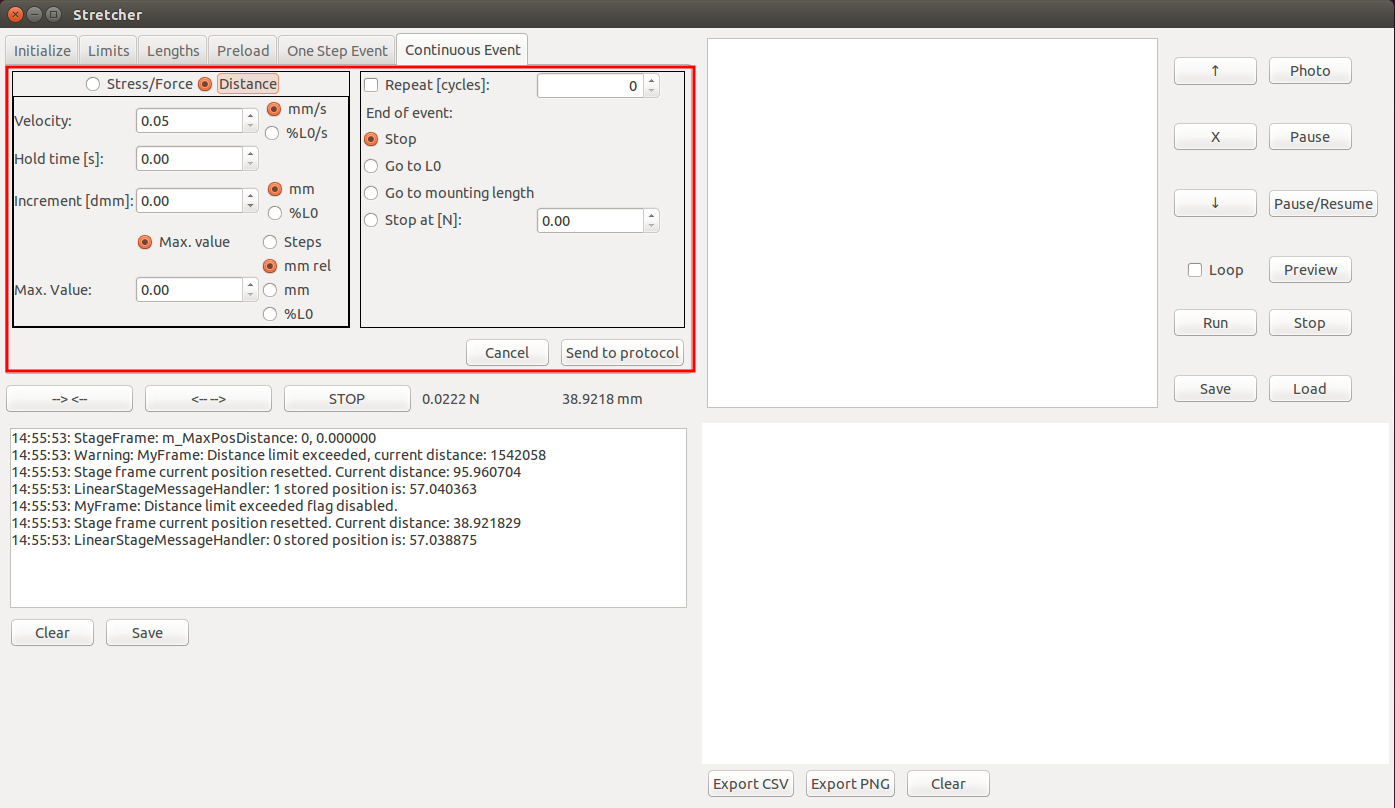
\includegraphics[width=1.0\textwidth]{images/ContinuousEventDistance}
	\caption{Continuous event experiment distance based}
	\label{fig:continuouseventdistance}
\end{figure}

\begin{figure}[!ht]
	\centering
		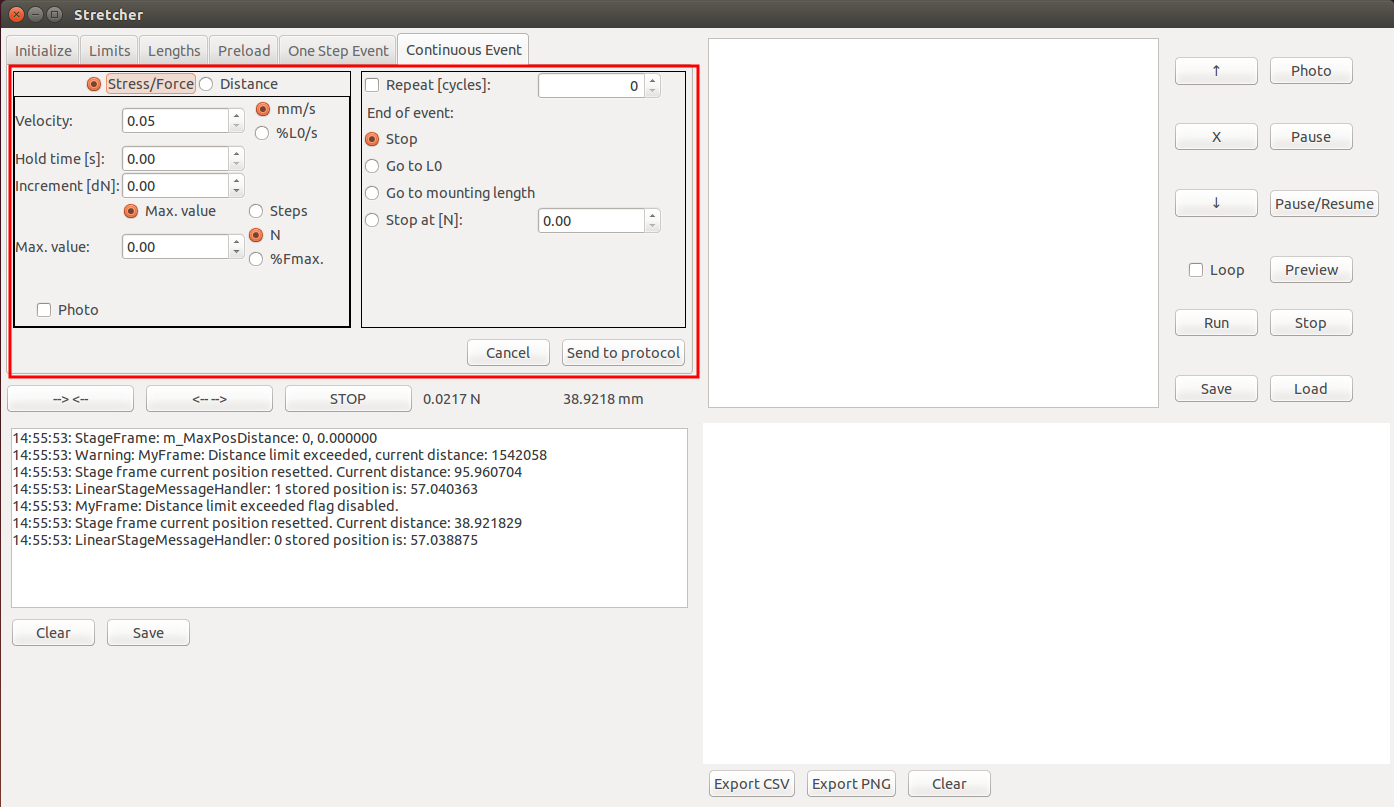
\includegraphics[width=1.0\textwidth]{images/ContinuousEventStressForce}
	\caption{Continuous event experiment force/stress based}
	\label{fig:continuouseventforcestress}
\end{figure}

\section{Pause}
The pause experiment is defined by only one parameter, the pause time. To add a pause experiment, the ``Pause button'', shown in figure \ref{fig:pause1} has to be pushed, which opens the pause dialog, shown in figure \ref{fig:pause2}. Here the pause time in seconds can be inserted and applied by pushing the button ``OK''.
\\
\\
In the pause experiment, nothing happens until the pause time is over and the next experiment can start.

\begin{figure}[!ht]
	\centering
		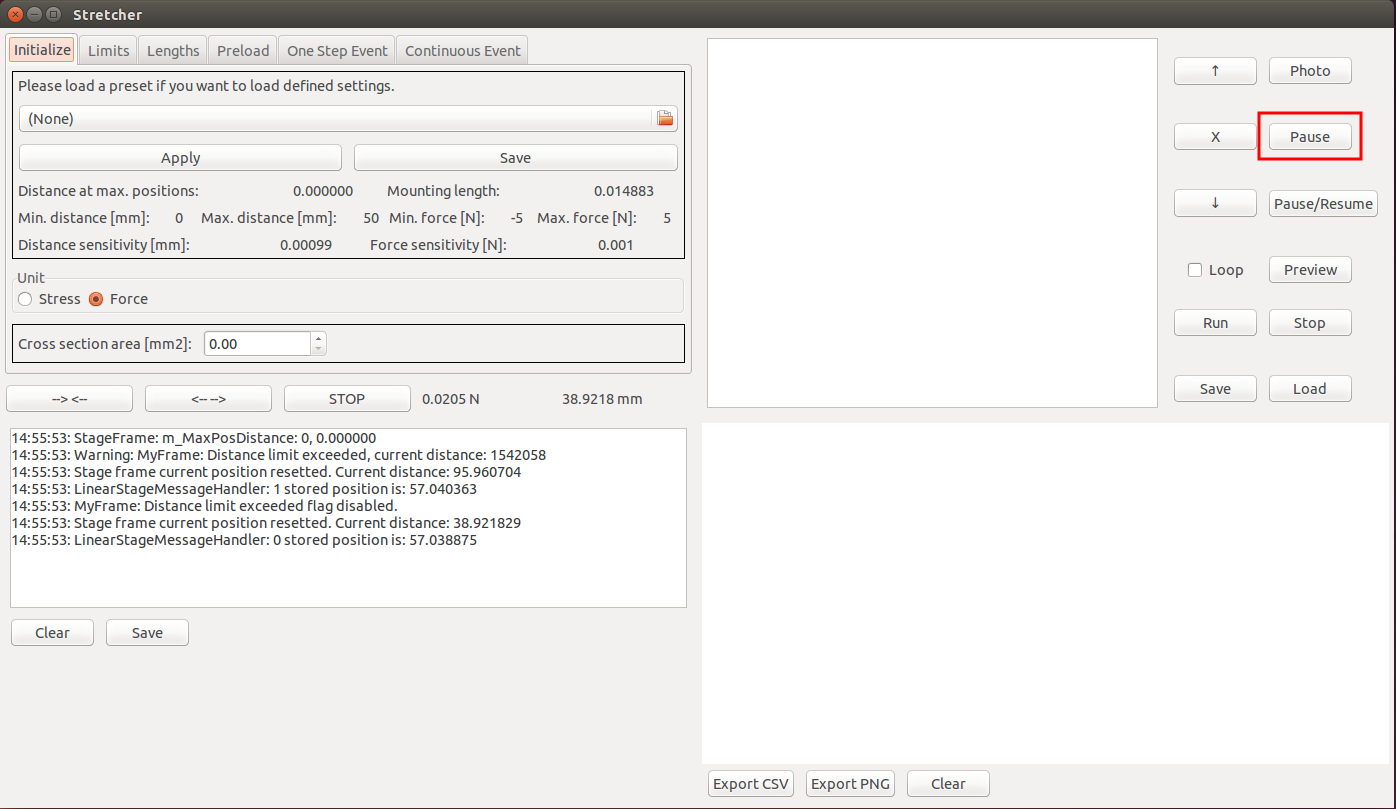
\includegraphics[width=1.0\textwidth]{images/Pause1}
	\caption{Pause experiment button}
	\label{fig:pause1}
\end{figure}

\begin{figure}[!ht]
	\centering
		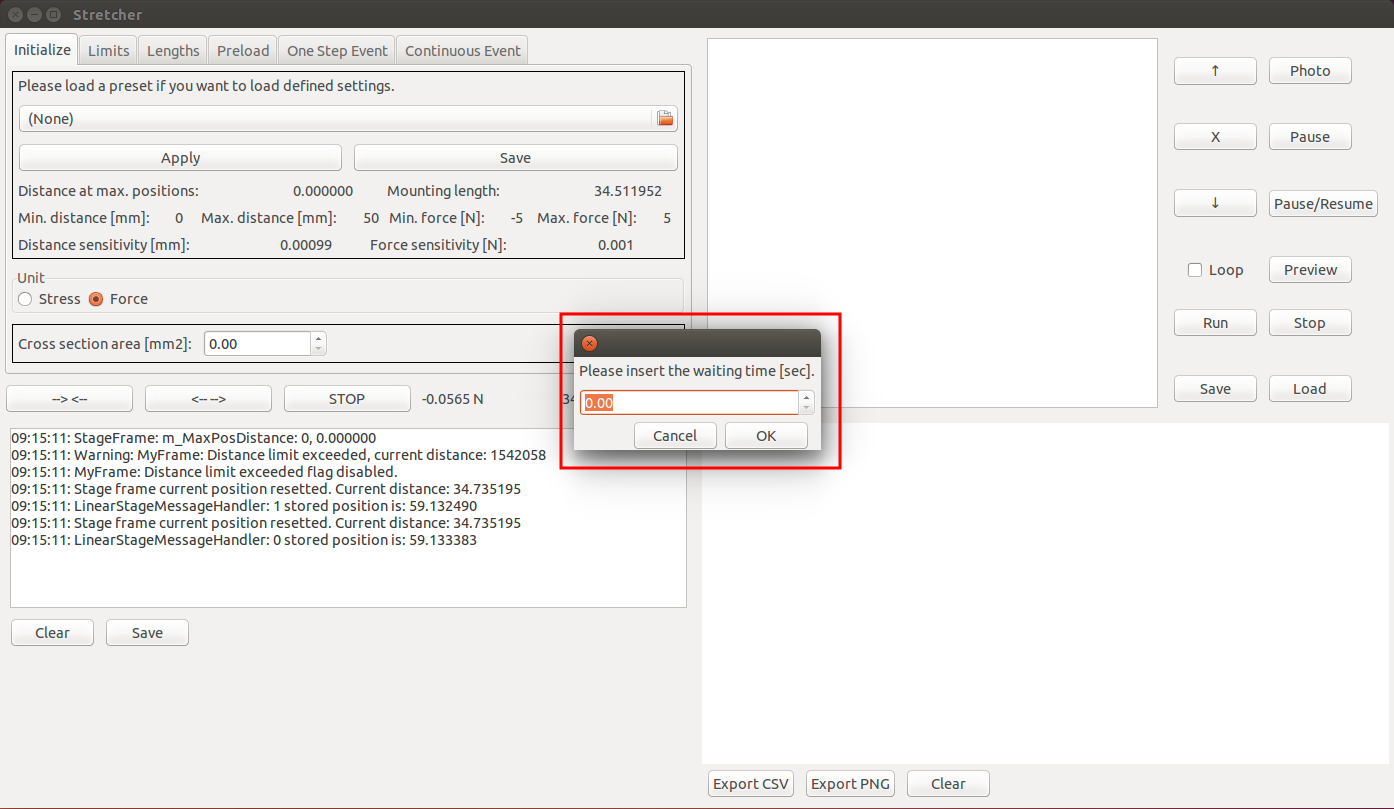
\includegraphics[width=1.0\textwidth]{images/Pause2}
	\caption{Pause experiment dialog}
	\label{fig:pause2}
\end{figure}

\section{Pause/Resume}
The pause/resume experiment doesn't have any parameters. To add a pause/resume experiment, the ``Pause/Resume'' button, shown in figure \ref{fig:pauseresume}, has to be pushed.
\\
\\
In the pause/resume experiment, a dialog will pop up and the experiment waits until the user continuous by pushing the button ``OK''.

\begin{figure}[!ht]
	\centering
		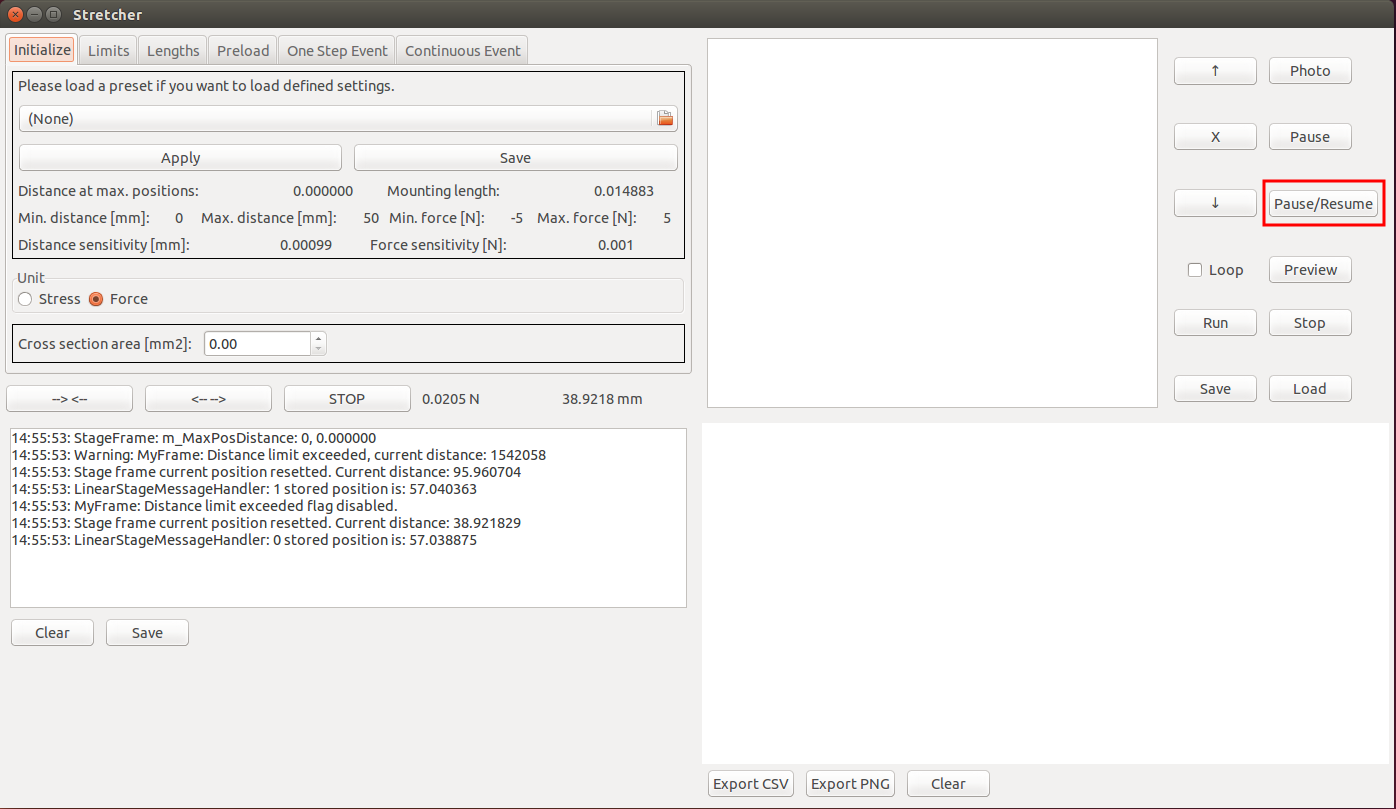
\includegraphics[width=1.0\textwidth]{images/PauseResume}
	\caption{Pause/resume experiment}
	\label{fig:pauseresume}
\end{figure}
